\section{Lektion 06-02-2018}

\begin{enumerate}
	\item Vinkel modulation
	\item Phasor repræsentation
\end{enumerate}

\begin{mdframed}[style=exampledefault]
	\begin{itemize}
		\item \textbf{Pensum:} JV, Ch 1 p 6-13, p 13-18
		\item \textbf{Opgaver:} P.I-2
	\end{itemize}
\end{mdframed}

\subsection{Vinkel modulation}
Vinkel modulation er processen når frekvensen eller phase af carrieren varrierer i forhold til baseband informationen. Her er amplituden $A_{c0}$ konstant. En vigtig fordel ved PM og FM modulation er at de mere imun overfor channel noise, nonlinear distotion og amplitude fading i forhold til AM modulation. Vinkel modulation kræver en dobbelt så stor båndbredde som AM modulation ($2\cdot W$). \\

\noindent Vinkel modulation er delt op i frekvens (\textbf{FM}) og phase (\textbf{PM}).

\begin{itemize}
	\item Vinkel modulation, $A(t) = A_{c0}$
	\begin{itemize}
		\item \textit{phase modulation, AM} ~\ref{eq:PM}
		\item \textit{frequency modulation, PM} ~\ref{eq:FM}
	\end{itemize}
\end{itemize} 

\begin{equation}\label{eq:PM}
y(t) = A_{c0} \cos(\omega_c t + \beta x(t))
\end{equation}

\begin{equation}\label{eq:FM}
y(t) = A_{c0} \cos(\omega_c t + \phi(t))
\end{equation}


\textit{The change in phase, changes the frequency of the modulated wave. The frequency of the wave also changes the phase of the wave.}

\begin{figure} [H]
	\centering
	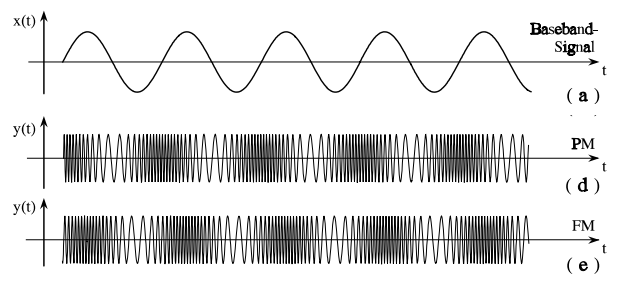
\includegraphics[width=\linewidth]{graphics/8.png}
	\caption{Examples of modulation waveshapes (PM and FM) from a sinusoidal baseband signal $x(t)$.}
	\label{fig:8}
\end{figure}

\begin{description}
	\item[$\beta$] $=\frac{\Delta f_{max}}{f_x}$ maximum phase deviation from the carrier phase
	\item[$\Delta f_{max}$] peak frequency deviation
\end{description}

\subsubsection{PM}

\begin{equation}\label{eq:PM1}
\theta(t) =\omega_c t +\beta x(t)+\phi_0
\end{equation}

\begin{description}
	\item[$x(t)$] Baseband signal
	\item[$\omega_c t$] Angle of Unmodulated carrier wave
	\item[$\beta$]$=\frac{radian}{volt}$ Phase sensitivity (const.)
	\item[$\phi_0$] $=0$ Initial angle
\end{description}

\subsubsection{FM}
\textbf{Indirect FM}
\begin{equation}\label{eq:FM1}
\theta_i(t) =\omega_c t + \beta \int_{}^{} x(t) dt
\end{equation}

\noindent \textbf{Direct FM}
\begin{equation}\label{eq:FM2}
\theta_i(t) =\omega_c t +2\pi K_V\int_{}^{} x(t) dt
\end{equation}

\begin{description}
	\item[$x(t)$] Baseband signal
	\item[$\omega_c t$] Angle of Unmodulated carrier wave
	\item[$\beta$]$=\frac{radian}{volt}$ Phase sensitivity (const.)
	\item[$K_V$]$=\frac{hertz}{volt}$ Frequency gain (const.)
\end{description}

\subsection{Phasor repræsentation}

\begin{figure} [H]
	\centering
	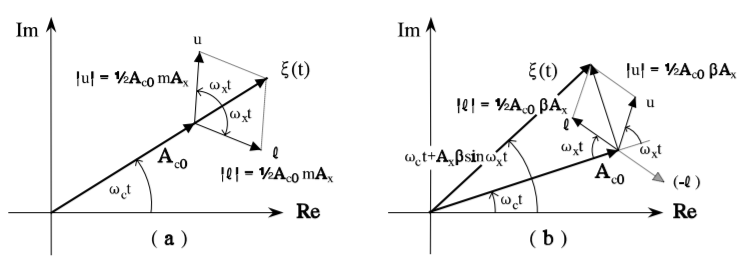
\includegraphics[width=\linewidth]{graphics/9.png}
	\caption{Phasor representation showing how the lower and upper sideband components, \textit{l}	and \textit{u}, add to the carrier $A_{c0}$ in (a) AM modulation, and (b) narrowband FM. The modulated wave becomes $y(t)=Re(\zeta)$.}
	\label{fig:9}
\end{figure}
